\subsection{Анализ цепи частотным методом при действии одиночного импульса на входе}

\newcommand{\abs}[1]{\left| #1 \right|}

Вычислим и построим 
графики АЧХ и ФЧХ функции передачи цепи 
$ H_U(j\omega) $.

$$ H_U(j\omega) = 
\left. H_U(s) \right|_{s = j\omega} =
\left| H_U(j\omega) \right|\,e^{j\,\Phi(\omega)}
$$

С учётом (\ref{eq:H_U_s}):

\begin{equation}\label{eq:H_U_j_omega}
H_U(j\omega) = 
\dfrac{4 + j\omega}{-2\omega^2 + 8j\omega + 4}
\end{equation}

Согласно свойству модулей комплексных чисел:

$$ |z_{1} \div z_{2}| = |z_{1}| \div |z_{2}| $$

АЧХ:

$
\abs{H_U(j\omega)} = 
\abs{\dfrac{4 + j\omega}{-2\omega^2 + 8j\omega + 4}} =
\dfrac{\abs{4 + j\omega}}{\abs{-2\omega^2 + 8j\omega + 4}} =
\dfrac{\sqrt{4^2+1^2}}{\sqrt{(4-2\omega^2)^2 + (8\omega)^2}}
$\\\\

\begin{equation}\label{eq:ach}
    \abs{H_U(j\omega)} = 
    \sqrt{\dfrac{17}{(4-2\omega^2)^2 + (8\omega)^2}}
\end{equation}

График АЧХ представлен на рис. \ref{fig:ach}

\begin{figure}[H]
    \centering
    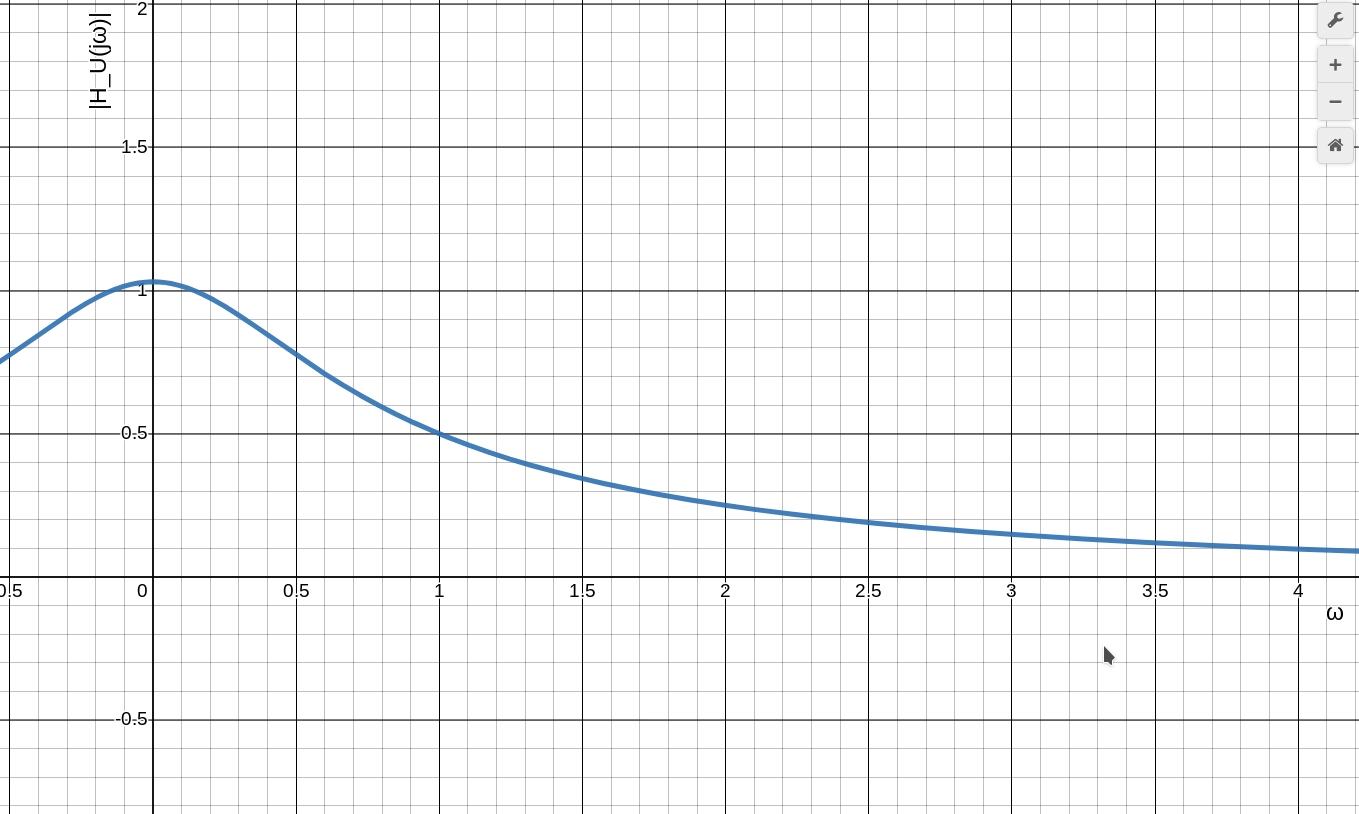
\includegraphics[width=0.7\linewidth]{photo/ach}
    \caption{График АЧХ}
    \label{fig:ach}
\end{figure}

ФЧХ:

Воспользуемся свойством
агрумента частного
комплексных чисел:

\textit{Аргумент частного двух комплексных чисел 
равен разности аргументов делимого и делителя.}

$$ \arg\left(\dfrac{z_1}{z_2}\right) = \arg(z_1) - \arg(z_2) $$

$
\Phi(\omega) = 
\arg\left(
    \dfrac{4 + j\omega}{-2\omega^2 + 8j\omega + 4}
\right) = 
\arg(4 + j\omega) - \arg((4 - 2\omega^2) + 8j\omega) =
\arctg\left(
    \dfrac{\omega}{4}
\right) - 
\arctg\left(
    \dfrac{8\omega}{4 - 2\omega^2}
\right)
$

\begin{equation}\label{eq:fch}
\Phi(\omega) = \arctg\left(
\dfrac{\omega}{4}
\right) - 
\arctg\left(
\dfrac{8\omega}{4 - 2\omega^2}
\right)
\end{equation}

График ФЧХ представлен на рис. \ref{fig:fch}

\begin{figure}[H]
    \centering
    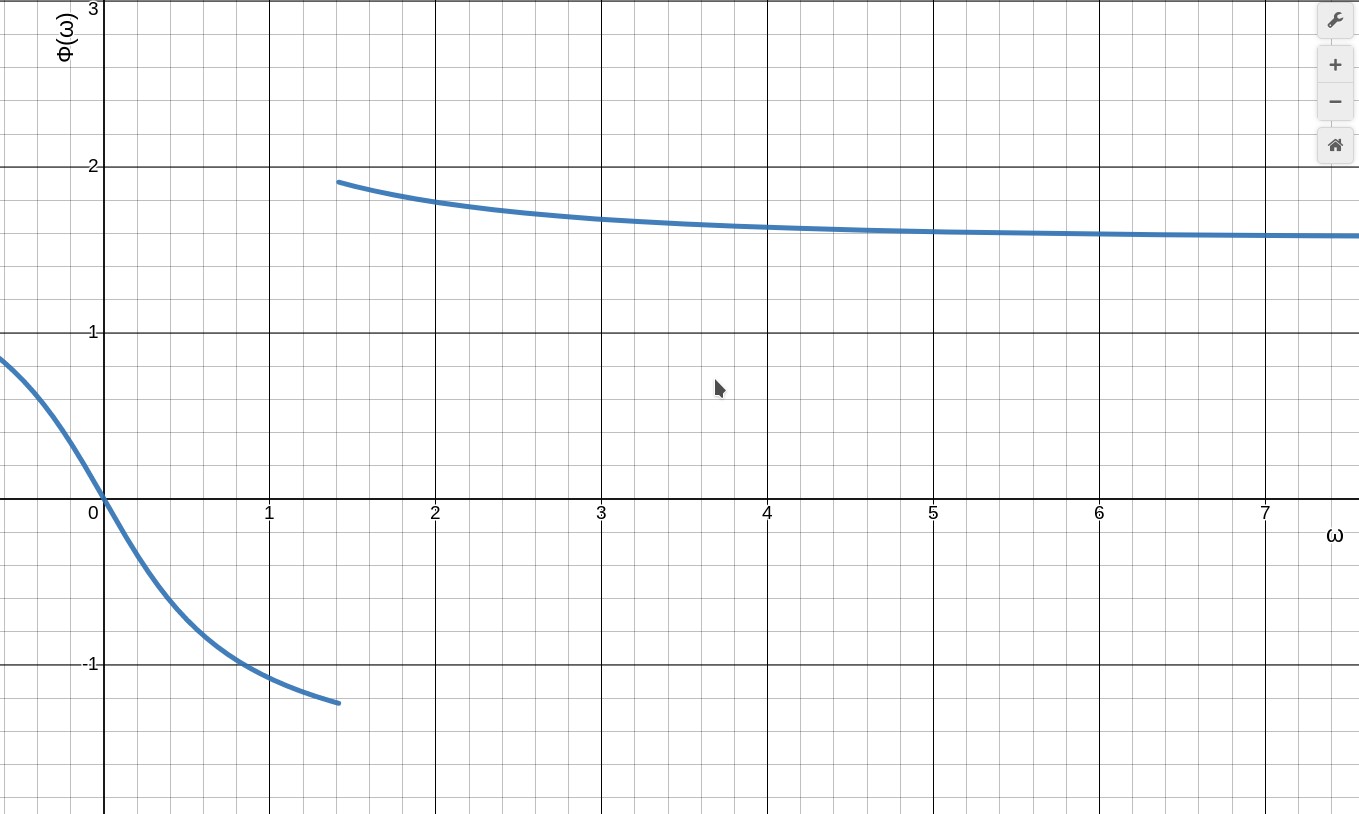
\includegraphics[width=0.7\linewidth]{photo/fch}
    \caption{График ФЧХ}
    \label{fig:fch}
\end{figure}

Найдём полосу пропускания.

Полоса пропускания определяется как диапазон частот, 
в котором
$ |H_U(j\omega)| \ge 0.707\,|H_U(j\omega)|_{\max} $
\\

Исходя из графика (рис. \ref{fig:ach}):

$$ |H_U(j\omega)|_{\max} = |H_U(0)| = 1.03 $$

$$ \Delta\omega \simeq 0.707 \cdot 1.03 \simeq 0.728 \; с^{-1} $$
